\section{hash functions}

\begin{frame}
	%\frametitle{Was sie tun}
	\frametitle{what they do}
	%Eigenschaften
	Propertys:
	\begin{columns}
	\column{6cm}
		\begin{itemize}
		%	\item Surjektiv \begin{small}(Eindeutige Abbildung)\end{small}
		%	\item Kollisionsfrei
		%	\item Lawineneffekt
			\item surjective \begin{small}(unambiguous projection)\end{small}
			\item collision free
			\item good averlancheffect
		\end{itemize}
	\column{6cm}
		\begin{center}
			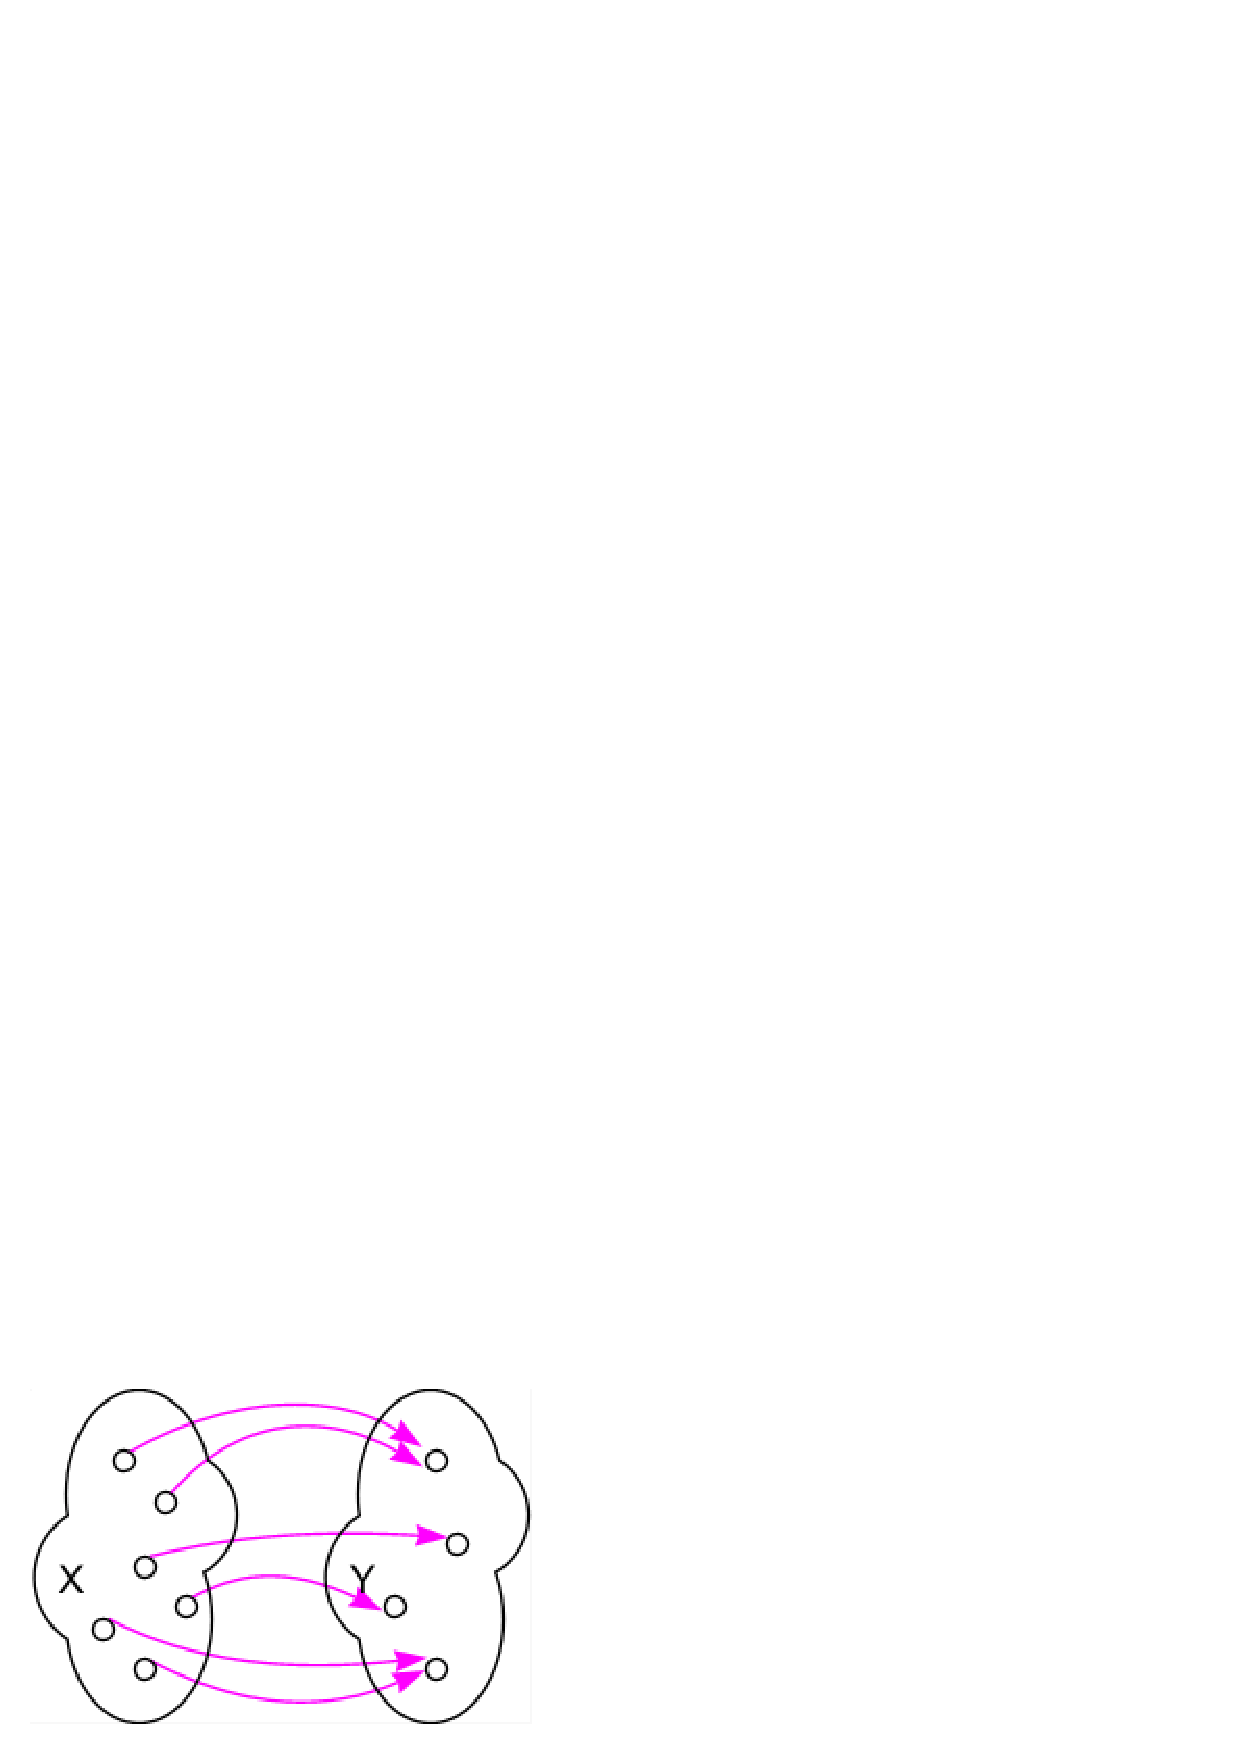
\includegraphics[width=4.8cm,height=3.2cm]{surjektiv}
		\end{center}
	\end{columns}
\end{frame}

\begin{frame}
\frametitle{what for?}
	\begin{columns}
	\column{6cm}
		\begin{itemize}
			\item One-way property
			\item usefull for large messages
		\end{itemize}
	\column{6cm}
		\begin{center}
			
\includegraphics[width=4cm,height=6cm]{oneway}
		\end{center}
	\end{columns}
\end{frame}

\begin{frame}
\frametitle{example of usage (1)}
	secure storage of passwords
	\par
	\begin{center}$hash( seed \parallel passwort )$\end{center}
\end{frame}

\begin{frame}
	\frametitle{example of usage (2)}
	Alice and Bob want to make a decission, where there normaly would flip a coin for.
	But they can not meet and have only a halfduplex communication channel (ex. a telephoneline).
	\begin{enumerate}
		\item Alice generates a random bitstring $m$ of sufficient length (ex. 512 bit) and keeps it secret
		\item Alice sends Bob the hash value $h(m)$ of $m$
		\item Bob ''guesse'' the value of the least significant (or other well defined) bit and sends his guess to Alice
		\item Alice now sends $m$ to Bob
		\item Bob validates that the recieved hash matches the hash of the recieved bitstring $m$
	\end{enumerate}	
\end{frame}

\begin{frame}
\frametitle{Attacs}
	\begin{itemize}
		\item Rainbow tables (time/memory tradeoff)
		\item brute-force (z.B. A..z, 0..9)
		\item analytical attacs
	\end{itemize}
\end{frame}

\begin{frame}
\frametitle{counter measurements (1)}
	\large{always use salts!}
\end{frame}

\begin{frame}
\frametitle{countermesaurements (2)}
	concatenation of different hash functions:
	\par
	\begin{center}$hash_1 (msg) \parallel hash_2(msg)$\end{center}
\end{frame}

